\section{Problem 3-7}
\label{sec:problem7}

Given $\vect{r}(t_0)$, $\ivect{v}(t_0)$ at $t_0 = 21.02$ min for Case 5, the same Kepler-equation solver is used to find $E$, $\nu$, and $\vect{r}(t)$, $\ivect{v}(t)$ at $t = 1913.38$ min, with $\mu = 398600~\text{km}^3\cdot\text{s}^{-2}$, and the result is compared to \texttt{ode113} at $t_f$ and over a 100-subinterval time series.

\programoutput{outputs/problem7.txt}

The Kepler solution agrees with \texttt{ode113} to within $5.7\times10^{-6}$~km in position and $2.3\times10^{-9}$~km/s in velocity at $t_f$.

\begin{figure}[H]
    \centering
    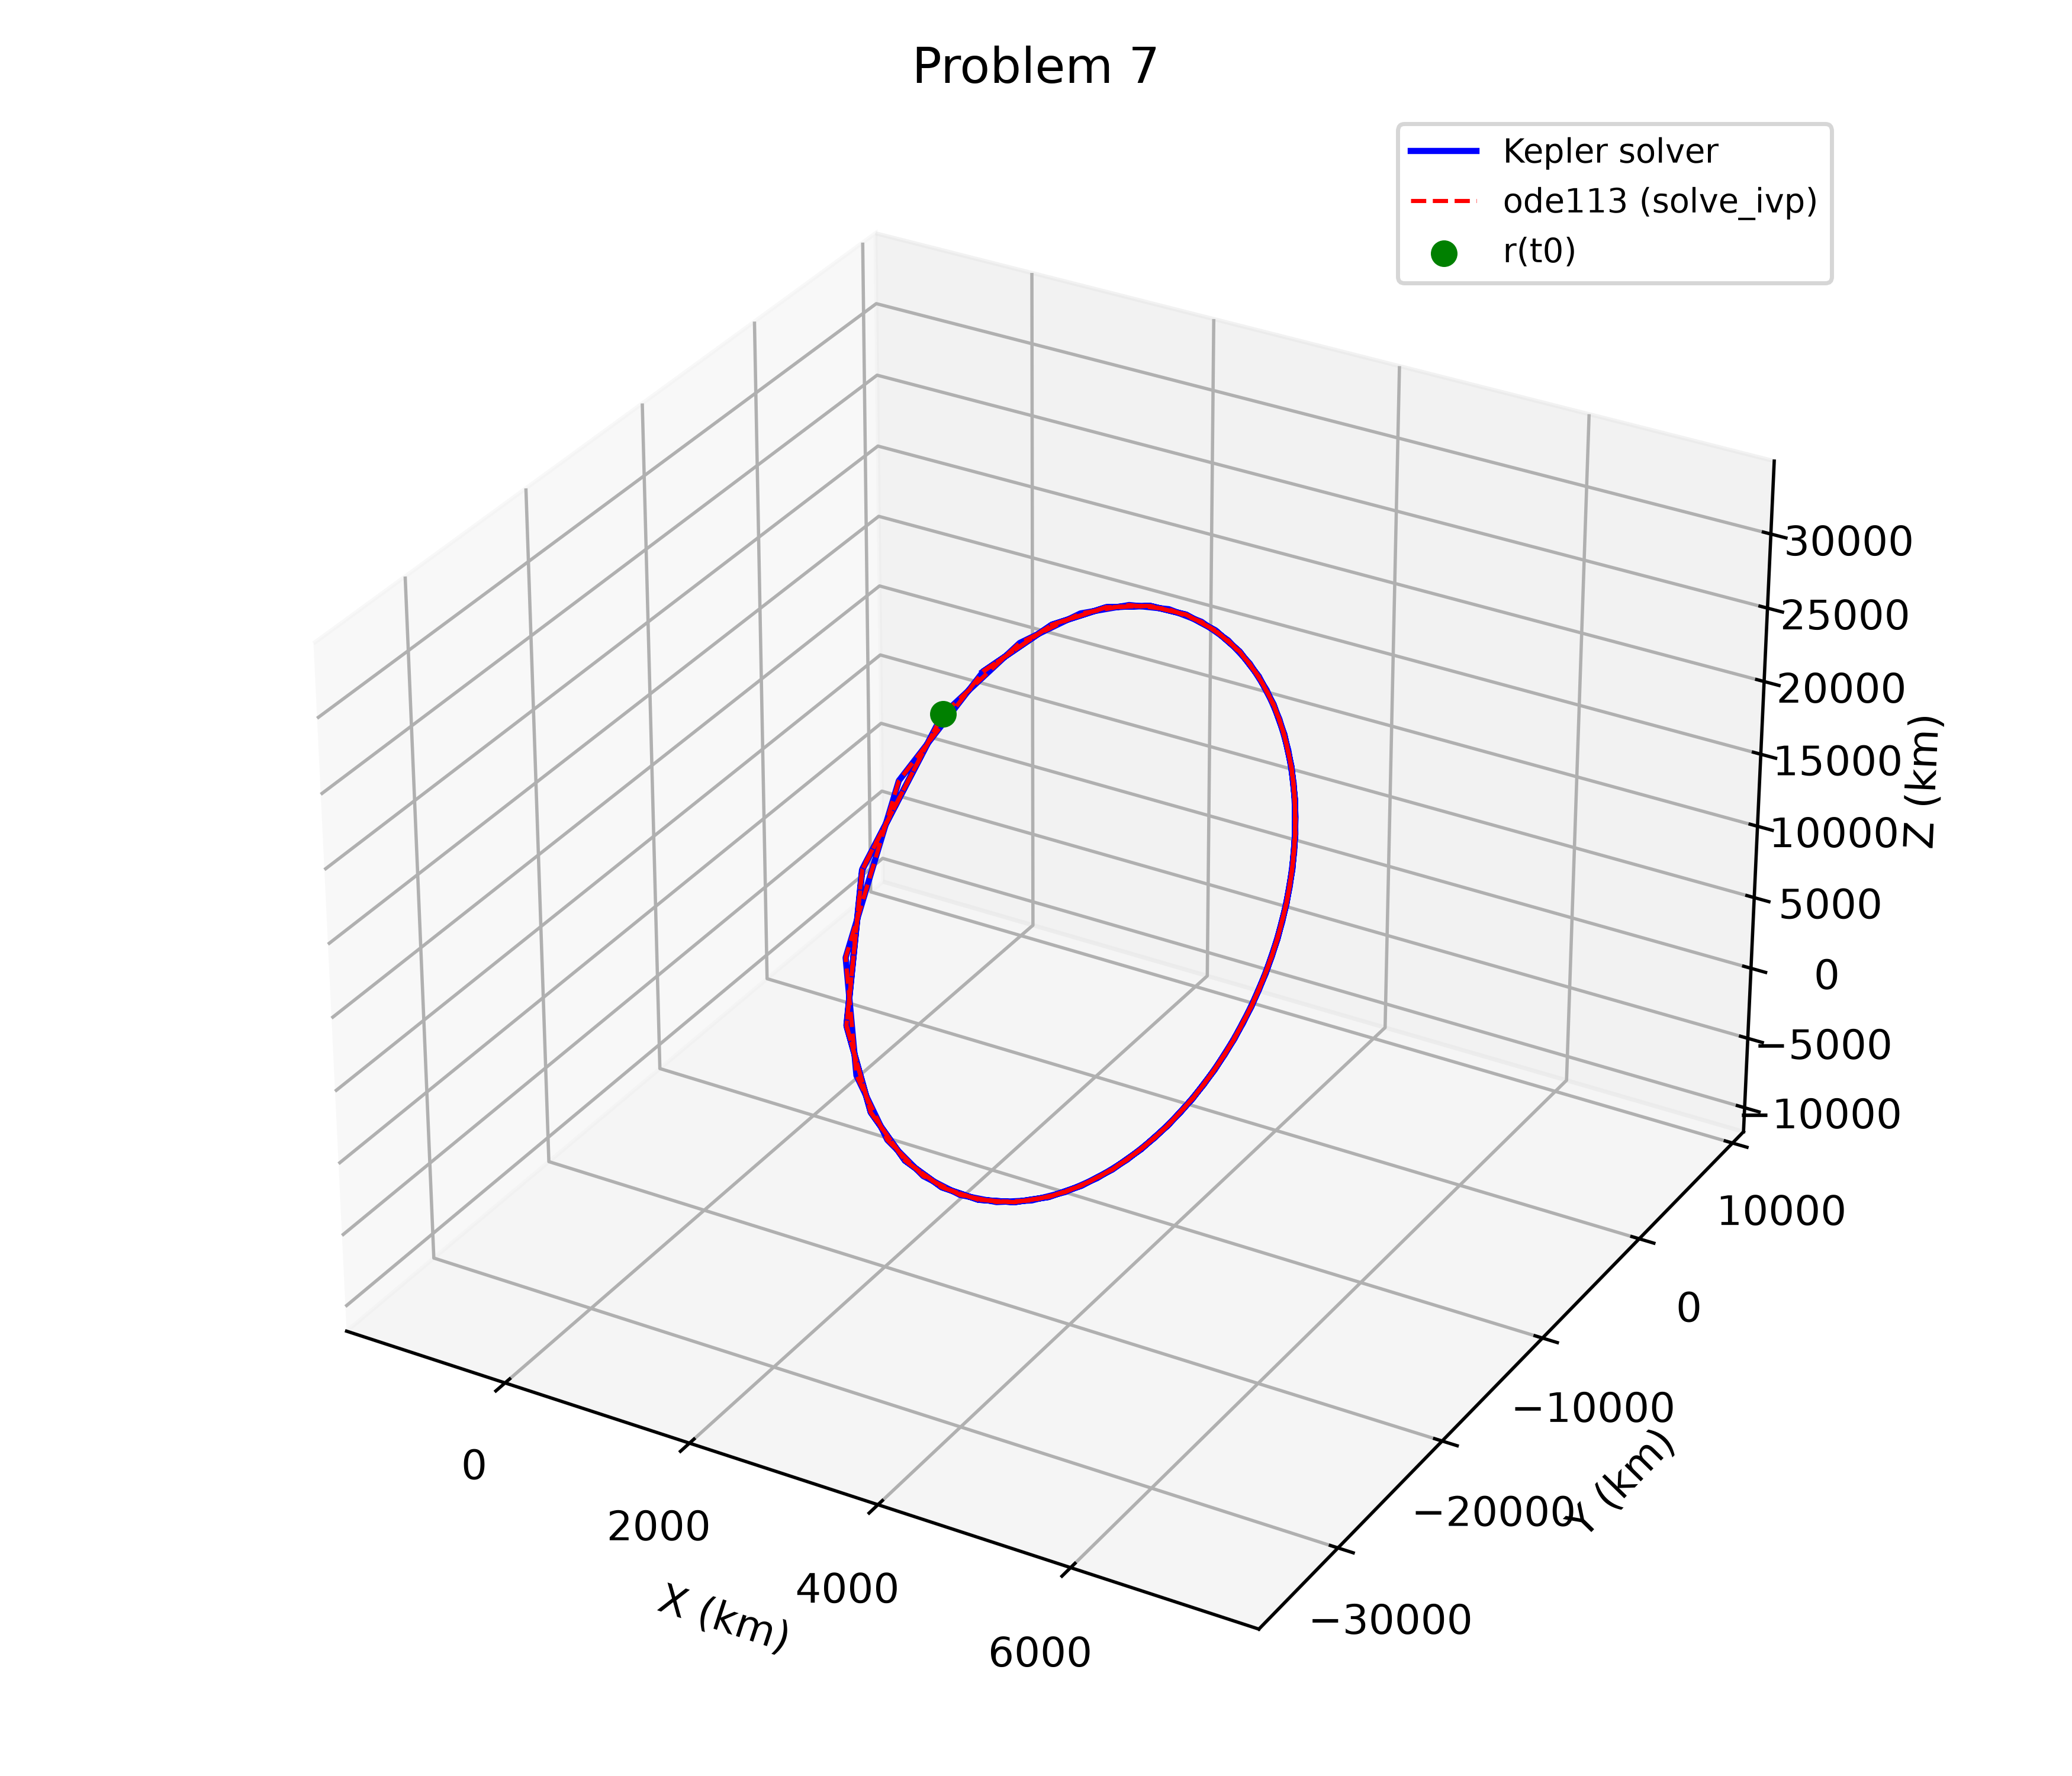
\includegraphics[width=0.75\textwidth]{figures/problem7_orbit.png}
    \caption{PCI position time series from the Kepler solver compared to \texttt{ode113}, Problem 3-7.}
\end{figure}

\FloatBarrier
